\documentclass[letterpaper,10pt]{article}

\usepackage[margin=1in]{geometry}

\usepackage{amsthm,amssymb,amsmath}
%% H/T: https://tex.stackexchange.com/a/202168/32270
\usepackage{textcomp}
%% H/T: https://tex.stackexchange.com/a/56877/32270
\usepackage{algorithm}
\usepackage{algpseudocode}
%% H/T: https://tex.stackexchange.com/a/244805
\usepackage{booktabs,siunitx}
%% H/T: https://tex.stackexchange.com/a/4217/32270
\usepackage{mathtools}

\theoremstyle{definition}
\newtheorem{theorem}{Theorem}

\usepackage[usenames, dvipsnames]{color}
\usepackage{hyperref}
\hypersetup{
  colorlinks=true,
  urlcolor=blue,
  linkcolor=MidnightBlue,
  citecolor=ForestGreen,
  pdfinfo={
    CreationDate={D:20180425160342},
    ModDate={D:20180425160342},
  },
}

%% H/T: https://tex.stackexchange.com/a/99051/32270
\PassOptionsToPackage{usenames,dvipsnames}{xcolor}
\usepackage{tikz}
\usetikzlibrary{shapes.geometric, arrows}
\tikzstyle{box} = [
  rectangle, minimum width=0.1\textwidth, minimum height=0.1\textwidth,
  text centered, draw=black]
\tikzstyle{empty-box} = [
  rectangle, minimum width=0.1\textwidth, minimum height=0.1\textwidth,
  text width=0.05\textwidth]
\tikzstyle{empty-box-vert} = [
  rectangle, minimum width=0.1\textwidth, minimum height=0.1\textwidth,
  text centered, text height=0.001\textwidth]
\tikzstyle{line} = [draw, -latex']

\usepackage{embedfile}
\embedfile{\jobname.tex}

\usepackage{fancyhdr}
\pagestyle{fancy}
\lhead{\(K\)-compensated de Casteljau}
\rhead{Danny Hermes}

\renewcommand{\headrulewidth}{0pt}
\newcommand{\cond}[1]{\operatorname{cond}\left(#1\right)}
\newcommand{\fl}[1]{\operatorname{fl}\left(#1\right)}
\newcommand{\eps}{\varepsilon}
\newcommand{\mach}{\mathbf{u}}

\begin{document}

\begin{abstract}
In computer aided geometric design a polynomial is usually represented in
Bernstein form. This paper presents a family of compensated algorithms to
accurately evaluate a polynomial in Bernstein form with floating point
coefficients. The principle is to apply error-free transformations to
improve the traditional de Casteljau algorithm. At each stage of computation,
round-off error is passed on to first order errors, then to second order
errors, and so on. After the computation has been ``filtered'' \((K - 1)\)
times via this process, the resulting output is as accurate as the de Casteljau
algorithm performed in \(K\) times the working precision. Forward error
analysis and numerical experiments illustrate the accuracy of this family
of algorithms.
\end{abstract}

\tableofcontents

\section{Introduction}

In computer aided geometric design, polynomials are usually expressed in
Bernstein form. Polynomials in this form are usually evaluated by the
de Casteljau algorithm. This algorithm has a round-off error bound
which grows only linearly with degree, even though the number of
arithmetic operations grows quadratically. Nevertheless the de Casteljau
algorithm returns results arbitrarily less accurate than the working
precision \(\mach\) when evaluating \(p(s)\) is ill-conditioned.
The relative accuracy of the computed
evaluation with the de Casteljau algorithm (\texttt{DeCasteljau}) satisfies
(\cite{Mainar1999}) the following a priori bound:
\begin{equation}\label{de-casteljau-error}
  \frac{\left|p(s) - \mathtt{DeCasteljau}(p, s)\right|}{\left|p(s)\right|} \leq
  \cond{p, s} \times \mathcal{O}(\mach).
\end{equation}
In the right-hand side of this inequality, \(\mach\) is the computing
precision and the condition number \(\cond{p, s} \geq 1\) only depends
on \(s\) and the Bernstein coefficients of \(p\) --- its expression will
be given further.

For ill-conditioned problems, such as evaluating \(p(s)\) near a
multiple root, the condition number may be arbitrarily large, i.e.
\(\cond{p, s} > 1 / \mach\), in
which case most or all of the computed digits will be incorrect.
In some cases, even the order of magnitude of the computed value
of \(p(s)\) can be incorrect.

To address ill-conditioned problems, error-free transformations (EFT) can
be applied in \textit{compensated algorithms} to account for roundoff.
Error-free transformations were studied in great detail in \cite{Ogita2005}
and open a large number of applications.
In \cite{langlois_et_al:DSP:2006:442}, a compensated Horner's algorithm was
described to evaluate a polynomial in the monomial basis. In \cite{Jiang2010},
a similar method was described to perform a compensated version of the de
Casteljau algorithm. In both cases, the \(\cond{p, s}\) factor is moved
from \(\mach\) to \(\mach^2\) and the computed value is as accurate
as if the computations were done in twice the working precision. For example,
the compensated de Casteljau algorithm (\texttt{CompDeCasteljau}) satisfies
\begin{equation}\label{de-casteljau-2-error}
  \frac{\left|p(s) - \mathtt{CompDeCasteljau}(p, s)\right|}{
    \left|p(s)\right|} \leq \mach + \cond{p, s} \times
    \mathcal{O}\left(\mach^2\right).
\end{equation}
For problems with \(\cond{p, s} < 1 / \mach^2\), the relative error
is \(\mach\), i.e. accurate to full precision, aside from rounding to the
nearest floating point number. Figure~\ref{fig:jlcs-10} shows this shift
in relative error from \texttt{DeCasteljau} to \texttt{CompDeCasteljau}.

\begin{figure}
  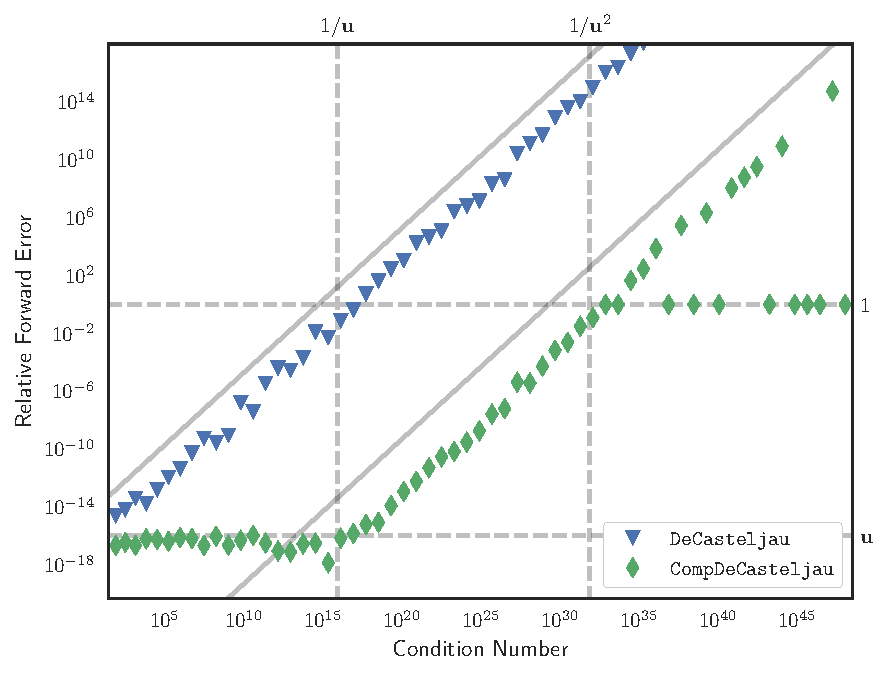
\includegraphics[width=0.8125\textwidth]{../images/jlcs10_plot.pdf}
  \centering
  \caption{Evaluation of \(p(s) = (s - 1)\left(s - 3/4\right)^7\)
    represented in Bernstein form.}
  \label{fig:jlcs-10}
\end{figure}

In \cite{Graillat2009}, the authors built on the compensated Horner's
algorithm to produce a method for evaluating a polynomial as if
the computations were done in \(K\) times the working precision for
any \(K \geq 2\). This result motivates this paper, though the
approach there is somewhat different than ours. They perform each computation
with error-free transformations and interpret the errors as coefficients of new
polynomials. They then evaluate the error polynomials, which (recursively)
generate second order error polynomials and so on. This recursive property
causes the number of operations to grow exponentially in \(K\). Here, we
instead have a fixed number of error groups, each corresponding to roundoff
from the group above it. For example, when
\((1 - s) b_j^{(n)} + s b_{j + 1}^{(n)}\) is computed in floating point, any
error is filtered down to the error group below it.

As in~\eqref{de-casteljau-error}, the accuracy of the compensated
result~\eqref{de-casteljau-2-error} may be arbitrarily bad for ill-conditioned
polynomial evaluations. For example, as the condition number grows in
Figure~\ref{fig:jlcs-10}, some points have relative error exactly equal to
\(1\); this indicates that \(\mathtt{CompDeCasteljau}(p, s) = 0\), which is
a complete failure to evaluate the order of magnitude of \(p(s)\).
We describe how to defer rounding into progressively
smaller error groups and improve the accuracy of the computed result by a
factor of \(\mach\) for every error group added. So we derive
\texttt{CompDeCasteljauK}, a \(K\)-fold compensated de Casteljau algorithm
that satisfies the following a prior bound for any arbitrary integer \(K\):
\begin{equation}
  \frac{\left|p(s) - \mathtt{CompDeCasteljauK}(p, s)\right|}{
    \left|p(s)\right|} \leq \mach + \cond{p, s} \times
    \mathcal{O}\left(\mach^K\right).
\end{equation}
This means that the computed value with \texttt{CompDeCasteljauK} is now
as accurate as the result of the de Casteljau algorithm performed in
\(K\) times the working precision with a final rounding back to this
working precision.

The paper is organized as follows. Section~\ref{sec:notation} introduces some
basic notation and results about floating point arithmetic, error-free
transformations and the de Casteljau algorithm. In
Section~\ref{sec:compensated-2},
the compensated algorithm for polynomial evaluation from \cite{Jiang2010} is
reviewed and notation is established for the expansion. In
Section~\ref{sec:compensated-k}, the \(K\) compensated algorithm is provided and
a forward error analysis is performed. Finally, in Section~\ref{sec:numerical} we
give numerical tests to illustrate the practical efficiency of our algorithms.

\section{Basic notation and results}\label{sec:notation}

Throughout this paper we assume that the computation in floating point
arithmetic obeys the model
\begin{equation}
  a \star b = \fl{a \circ b} = (a \circ b)(1 + \eps_1) =
  (a \circ b) / (1 + \eps_2)
\end{equation}
where \(\star \in \left\{\oplus, \ominus, \otimes, \oslash\right\}\), \(\circ
\in \left\{+, -, \times, \div\right\}\) and \(\left|\eps_1\right|,
\left|\eps_2\right| \leq \mach\). The symbol \(\mach\) is the unit round-off
and \(\star\) represents the floating point computation, e.g.
\(a \oplus b = \fl{a + b}\). We also assume that the computed result of
\(\alpha \in \mathbf{R}\) in floating point arithmetic is denoted by
\(\widehat{\alpha}\) or \(\fl{\alpha}\) and \(\mathbf{F}\) denotes the set of
all floating point numbers (see \cite{Higham2002} for more details).
Following \cite{Higham2002}, we will use the following classic properties in
error analysis.

\begin{enumerate}
  \item If \(\delta_i \leq \mach\), \(\rho_i = \pm 1\), then
      \(\prod_{i = 1}^n (1 + \delta_i)^{\rho_i} = 1 + \theta_n\),
  \item \(\left|\theta_n\right| \leq \gamma_n \coloneqq
      n \mach / (1 - n \mach)\),
  \item \((1 + \theta_k)(1 + \theta_j) \leq (1 + \theta_{k + j})\),
  \item \(\gamma_k + \gamma_j + \gamma_k \gamma_j \leq \gamma_{k + j}\),
  \item \((1 + \mach)^j \leq 1 / (1 - j \mach)\).
\end{enumerate}

Now let us introduce some results concerning error-free transformation (EFT).
For a pair floating point numbers \(a, b \in \mathbf{F}\), there exists
a floating point number \(y\) satisfying \(a \circ b = x + y\) where
\(x = \fl{a \circ b}\) and \(\circ \in \left\{+, -, \times\right\}\).
The transformation \((a, b) \longrightarrow (x, y)\) is regarded as an
error-free transformation. The error-free transformation algorithms of the
sum and product of two floating point numbers used later in this paper are
the \texttt{TwoSum} algorithm by Knuth \cite{Knuth1997} and \texttt{TwoProd}
algorithm by Dekker \cite{Dekker1971}, respectively. The following theorem
exhibits the important properties of \texttt{TwoSum} and \texttt{TwoProd}
algorithms (see \cite{Ogita2005}).

\begin{theorem}[\cite{Ogita2005}]
For \(a, b \in \mathbf{F}\) and \(P, \pi, S, \sigma \in \mathbf{F}\),
\texttt{TwoSum} and \texttt{TwoProd} satisfy
\begin{itemize}
  \item \(\left[S, \sigma\right] = \mathtt{TwoSum}(a, b)\), \(x = \fl{a + b}\),
      \(S + \sigma = a + b\), \(\sigma \leq \mach \left|S\right|\),
      \(\sigma \leq \mach \left|a + b\right|\)
  \item \(\left[P, \pi\right] = \mathtt{TwoProd}(a, b)\),
      \(P = \fl{a \times b}\), \(P + \pi = a \times b\),
      \(\pi \leq \mach \left|P\right|\),
      \(\pi \leq \mach \left|a \times b\right|\).
\end{itemize}
The letters \(\sigma\) and \(\pi\) are used to indicate that the
errors came from sum and product, respectively.
\end{theorem}

Next, we recall the de Casteljau algorithm:

\begin{algorithm}[H]
  \caption{\textit{de Casteljau algorithm for polynomial evaluation.}}

  \begin{algorithmic}
    \Function{\(\mathtt{res} = \mathtt{DeCasteljau}\)}{$b, s$}
      \State \(n = \texttt{length}(b) - 1\)
      \State \(\widehat{r} = 1 \ominus s\)
      \\
      \For{\(j = 0, \ldots, n\)}
        \State \(\widehat{b}_j^{(n)} = b_j\)
      \EndFor
      \\
      \For{\(k = n - 1, \ldots, 0\)}
        \For{\(j = 0, \ldots, k\)}
          \State \(\widehat{b}_j^{(k)} = \left(
              r \otimes \widehat{b}_j^{(k + 1)}\right) \oplus
              \left(s \otimes \widehat{b}_{j + 1}^{(k + 1)}\right)\)
        \EndFor
      \EndFor
      \\
      \State \(\mathtt{res} = \widehat{b}_0^{(0)}\)
    \EndFunction
  \end{algorithmic}
\end{algorithm}

\begin{theorem}[\cite{Mainar1999}]
If \(p(s) = \sum_{j = 0}^n b_j B_{j, n}(s)\) and \(\mathtt{DeCasteljau}(p, s)\)
is the value computed by the de Casteljau algorithm then
\begin{equation}
\left|p(s) - \mathtt{DeCasteljau}(p, s)\right| \leq \gamma_{2n}
\sum_{j = 0}^n \left|b_j\right| B_{j, n}(s).
\end{equation}
\end{theorem}

The relative condition number of the evaluation of \(p(s) = \sum_{j = 0}^n
b_j B_{j, n}(s)\) in Bernstein form used in this paper is (see
\cite{Mainar1999}, \cite{Farouki1987}):
\begin{equation}
\cond{p, s} = \frac{\widetilde{p}\left(s\right)}{
  \left|p(s)\right|} = \frac{\sum_j \left|b_j\right| B_{j, n}(s)}{
  \left|p(s)\right|},
\end{equation}
where \(B_{j, n} \geq 0\).

\section{Compensated de Casteljau}\label{sec:compensated-2}

In this section we review the compensated de Casteljau algorithm
from \cite{Jiang2010}. In order to track the local errors at
each update step, we use four EFTs:
\begin{align}
\left[\widehat{r}, \rho\right] &= \mathtt{TwoSum}(1, -s) \\
\left[P_1, \pi_1\right] &= \mathtt{TwoProd}\left(\widehat{r}, \widehat{b}_j^{(k + 1)}\right) \\
\left[P_2, \pi_2\right] &= \mathtt{TwoProd}\left(s, \widehat{b}_{j + 1}^{(k + 1)}\right) \\
\left[\widehat{b}_j^{(k)}, \sigma_3\right] &= \mathtt{TwoSum}(P_1, P_2)
\end{align}
With these, we can exactly describe the local error between the exact
update and computed update:
\begin{gather}
\ell_j^{(k)} = \pi_1 + \pi_2 + \sigma_3 + \rho\widehat{b}_j^{(k + 1)} \label{ell-j} \\
(1 - s) \cdot \widehat{b}_j^{(k + 1)} +
  s \cdot \widehat{b}_{j + 1}^{(k + 1)} =
\widehat{b}_j^{(k)} + \ell_j^{(k)}.
\end{gather}

\begin{figure}[H]
\centering
\begin{tikzpicture}[node distance = 0.2\textwidth]
  \node (b0) {\(\widehat{b}^{(n)}\)}
    child {node (b1) {\(\widehat{b}^{(n - 1)}\)}
      child {node (b2) {\(\widehat{b}^{(n - 2)}\)}
        child {node (bdots) {\(\vdots\)}
          child {node (bn) {\(\widehat{b}^{(0)}\)}}
          child {node (ln) {\(\ell^{(0)}\)}}
        }
        child {node (ldots) {\(\vdots\)}}
      }
      child {node (l2) {\(\ell^{(n - 2)}\)}}
    }
    child {node (l1) {\(\ell^{(n - 1)}\)}};
  %%
  \path (b1) -- (l1) node [midway] {\(+\)};
  \path (b2) -- (l2) node [midway] {\(+\)};
  \path (bn) -- (ln) node [midway] {\(+\)};
  %% eb == exact b
  \node [right of=b0] (eb0) {\(b^{(n)}\)}
    child {node (eb1) {\(b^{(n - 1)}\)}
      child {node (eb2) {\(b^{(n - 2)}\)}
        child {node (ebdots) {\(\vdots\)}
          child {node (ebn) {\(b^{(0)}\)}}
        }
      }
    };
\end{tikzpicture}
\caption{Local round-off errors}
\end{figure}

\noindent By defining the global errors at each step
\begin{equation}
  \partial b_j^{(k)} = b_j^{(k)} - \widehat{b}_j^{(k)}
\end{equation}
we can see that the local errors accumulate in
\(\partial b^{(k)}\):
\begin{equation}
  \partial b_j^{(k)} = (1 - s) \cdot \partial b_j^{(k + 1)} + s \cdot
  \partial b_{j + 1}^{(k + 1)} + \ell_j^{(k)}.
\end{equation}
Hence, when computed in exact arithmetic, we have
\begin{equation}
  p(s) = \widehat{b}_0^{(0)} + \partial b_0^{(0)}.
\end{equation}

The idea behind the compensated de Casteljau algorithm
is to compute both the local error and the updates of the global
error with floating point operations:

\begin{algorithm}[H]
  \caption{\textit{Compensated de Casteljau algorithm for polynomial evaluation.}}

  \begin{algorithmic}
    \Function{\(\mathtt{res} = \mathtt{CompDeCasteljau}\)}{$b, s$}
      \State \(n = \texttt{length}(b) - 1\)
      \State \(\left[\widehat{r}, \rho\right] = \mathtt{TwoSum}(1, -s)\)
      \\
      \For{\(j = 0, \ldots, n\)}
        \State \(\widehat{b}_j^{(n)} = b_j\)
        \State \(\widehat{\partial b}_j^{(n)} = 0\)
      \EndFor
      \\
      \For{\(k = n - 1, \ldots, 0\)}
        \For{\(j = 0, \ldots, k\)}
          \State \(\left[P_1, \pi_1\right] = \mathtt{TwoProd}\left(
              \widehat{r}, \widehat{b}_j^{(k + 1)}\right)\)
          \State \(\left[P_2, \pi_2\right] = \mathtt{TwoProd}\left(
              s, \widehat{b}_{j + 1}^{(k + 1)}\right)\)
          \State \(\left[\widehat{b}_j^{(k)}, \sigma_3\right] =
              \mathtt{TwoSum}(P_1, P_2)\)
          \State \(\widehat{\ell}_j^{(k)} = \pi_1 \oplus \pi_2 \oplus \sigma_3
              \oplus \left(\rho \otimes \widehat{b}_j^{(k + 1)}\right)\)
          \State \(\widehat{\partial b}_j^{(k)} =
              \left(\widehat{r} \otimes
              \widehat{\partial b}_j^{(k + 1)}\right) \oplus
              \left(s \otimes \widehat{\partial b}_{j + 1}^{(k + 1)}
              \right) \oplus
              \widehat{\ell}_j^{(k)}\)
        \EndFor
      \EndFor
      \\
      \State \(\mathtt{res} = \widehat{b}_0^{(0)} \oplus
          \widehat{\partial b}_0^{(0)}\)
    \EndFunction
  \end{algorithmic}
\end{algorithm}

\noindent  When comparing this computed error to the exact error, the
difference depends only on \(s\) and the Bernstein
coefficients of \(p\):

\begin{theorem}[\cite{Jiang2010}]
  If no underflow occurs and \(n \geq 2\), then
  \begin{equation}
    \left|\partial b_0^{(0)} - \widehat{\partial b}_0^{(0)}\right| \leq
    2 \gamma_{3n + 1} \gamma_{3(n - 1)}
    \sum_{j = 0}^n \left|b_j\right| B_{j, n}(s).
  \end{equation}
\end{theorem}

\noindent Using the bound on the error in \(\partial b\), the algorithm can
be shown to be as accurate as if the computations were done in twice
the working precision:

\begin{theorem}[\cite{Jiang2010}]
  If no underflow occurs, \(n \geq 2\) and \(s \in \left[0, 1\right]\)
  \begin{equation}
    \frac{\left|p(s) - \mathtt{CompDeCasteljau}(p, s)\right|}{\left|p(s)\right|} \leq \mach +
    2 \gamma_{3n}^2 \cond{p, s}.
  \end{equation}
\end{theorem}

\section{\texorpdfstring{\(K\)}{K} Compensated de Casteljau}\label{sec:compensated-k}

In order to raise from twice the working precision to \(K\) times the
working precision, we continue using EFTs when computing
\(\widehat{\partial b}^{(k)}\). By tracking the round-off from each
floating point evaluation via an EFT, we can form a cascade of global errors:
\begin{align}
  b_j^{(k)} &= \widehat{b}_j^{(k)} + \partial b_j^{(k)} \\
  \partial b_j^{(k)} &= \widehat{\partial b}_j^{(k)} + \partial^2 b_j^{(k)} \\
  \partial^2 b_j^{(k)} &= \widehat{\partial^2 b}_j^{(k)} +
  \partial^3 b_j^{(k)} \\
  & \vdots \nonumber
\end{align}
In the same way local error can be tracked when updating
\(\widehat{b}_j^{(k)}\), it can be tracked for updates that happen down
the cascade:
\begin{alignat}{4}
  (1 - s) \cdot \widehat{b}_j^{(k + 1)} &+
  s \cdot \widehat{b}_{j + 1}^{(k + 1)} &&  &&=
  \widehat{b}_j^{(k)} &&+ \ell_{1, j}^{(k)} \\
  (1 - s) \cdot \widehat{\partial b}_j^{(k + 1)} &+
  s \cdot \widehat{\partial b}_{j + 1}^{(k + 1)} &&+ \ell_{1, j}^{(k)} &&=
  \widehat{\partial b}_j^{(k)} &&+ \ell_{2, j}^{(k)} \\
  (1 - s) \cdot \widehat{\partial^2 b}_j^{(k + 1)} &+
  s \cdot \widehat{\partial^2 b}_{j + 1}^{(k + 1)} &&+ \ell_{2, j}^{(k)} &&=
  \widehat{\partial^2 b}_j^{(k)} &&+ \ell_{3, j}^{(k)} \\
  &  &&  &&\vdots && \nonumber
\end{alignat}

In \texttt{CompDeCasteljau}, after a single stage of error filtering we
``give up'' and use \(\widehat{\partial b}^{(k)}\) instead of
\(\partial b^{(k)}\) (without keeping around any information about the
round-off error). In order to obtain results that are as accurate as if
computed in \(K\) times the working precision, we must continue filtering
errors down \((K - 1)\) times, so that at the final level we compute
\(\widehat{\partial^{K - 1} b}^{(k)}\) and don't worry about round-off
error.

When computing \(\widehat{\partial^F b}\) (i.e. the error after
\(F\) stages of filtering)
there will be several sources of round-off. In particular, there will be
\begin{itemize}
\item errors when computing \(\widehat{\ell}_{F, j}^{(k)}\) from the
  terms in \(\ell_{F, j}^{(k)}\)
\item an error
for the ``missing'' \(\rho \cdot \widehat{\partial^F b}_j^{(k + 1)}\) in
\((1 - s) \cdot \widehat{\partial^F b}_j^{(k + 1)}\)
\item an error from the product
  \(\widehat{r} \otimes \widehat{\partial^F b}_j^{(k + 1)}\)
\item an error from the product
  \(s \otimes \widehat{\partial^F b}_{j + 1}^{(k + 1)}\)
\item two errors from the two \(\oplus\) when combining the three
  terms in
  \(\left[\widehat{r} \otimes \widehat{\partial^F b}_j^{(k + 1)}\right] \oplus
  \left[s \otimes \widehat{\partial^F b}_{j + 1}^{(k + 1)}\right] \oplus
  \widehat{\ell}_{F, j}^{(k)}\)
\end{itemize}
For example, in~\eqref{ell-j}:
\begin{equation}
\ell_{1, j}^{(k)} = \underbrace{\pi_1}_{P_1 = \widehat{r} \otimes
    \widehat{b}_j^{(k + 1)}} +
\underbrace{\pi_2}_{P_2 = s \otimes \widehat{b}_{j + 1}^{(k + 1)}} +
\underbrace{\sigma_3}_{P_1 \oplus P_2} +
\underbrace{\rho \cdot \widehat{b}_j^{(k + 1)}}_{(1 - s)
  \widehat{b}_j^{(k + 1)}}
\end{equation}
After each stage, we'll always have
\[\ell_{F, j}^{(k)} = e_1 + e_2 + \cdots + e_M + \rho \cdot
\widehat{\partial^{F - 1} b}_j^{(k + 1)}\]
where the terms \(e_1, \ldots, e_M\) come from using \texttt{TwoSum} and
\texttt{TwoProd} when computing \(\widehat{\partial^{F - 1} b}_j^{(k)}\)
and the \(\rho\) term comes from the roundoff
in \(1 \ominus s\) when multiplying \((1 - s)\) by
\(\widehat{\partial^{F - 1} b}_j^{(k + 1)}\). With this in mind, we
can define an EFT (\texttt{LocalErrorEFT}) that computes
\(\widehat{\ell}\) and tracks all round-off errors generated in
the process:

\begin{algorithm}[H]
  \caption{\textit{EFT for computing the local error.}}

  \begin{algorithmic}
    \Function{\(\left[\eta, \widehat{\ell}\right] =
        \mathtt{LocalErrorEFT}\)}{$e, \rho, \delta b$}
      \State \(M = \texttt{length}(e)\)
      \\
      \State \(\left[\widehat{\ell}, \eta_1\right] =
          \mathtt{TwoSum}(e_1, e_2)\)
      \For{\(j = 3, \ldots, M\)}
        \State \(\left[\widehat{\ell}, \eta_{j - 1}\right] =
            \mathtt{TwoSum}\left(\widehat{\ell}, e_j\right)\)
      \EndFor
      \\
      \State \(\left[P, \eta_M\right] =
          \mathtt{TwoProd}\left(\rho, \delta b\right)\)
      \State \(\left[\widehat{\ell}, \eta_{M + 1}\right] =
          \mathtt{TwoSum}\left(\widehat{\ell}, P\right)\)
    \EndFunction
  \end{algorithmic}
\end{algorithm}

\noindent With this EFT helper in place, we can perform \((K - 1)\)
error filtrations:

\begin{algorithm}[H]
  \caption{\(K\)-\textit{compensated de Casteljau algorithm.}}

  \begin{algorithmic}
    \Function{\(\mathtt{res} = \mathtt{CompDeCasteljau}\)}{$b, s$}
      \State \(n = \texttt{length}(b) - 1\)
      \State \(\left[\widehat{r}, \rho\right] = \mathtt{TwoSum}(1, -s)\)
      \\
      \For{\(j = 0, \ldots, n\)}
        \State \(\widehat{b}_j^{(n)} = b_j\)
        \For{\(F = 1, \ldots, K - 1\)}
          \State \(\widehat{\partial^F b}_j^{(n)} = 0\)
        \EndFor
      \EndFor
      \\
      \For{\(k = n - 1, \ldots, 0\)}
        \For{\(j = 0, \ldots, k\)}
          \State \(\left[P_1, \pi_1\right] = \mathtt{TwoProd}\left(
              \widehat{r}, \widehat{b}_j^{(k + 1)}\right)\)
          \State \(\left[P_2, \pi_2\right] = \mathtt{TwoProd}\left(
              s, \widehat{b}_{j + 1}^{(k + 1)}\right)\)
          \State \(\left[\widehat{b}_j^{(k)}, \sigma_3\right] =
              \mathtt{TwoSum}(P_1, P_2)\)
          \\
          \State \(e = \left[\pi_1, \pi_2, \sigma_3\right]\)
          \State \(\delta b = \widehat{b}_j^{(k + 1)}\)
          \\
          \For{\(F = 1, \ldots, K - 2\)}
            \State \(\left[\eta, \widehat{\ell}\right] =
                \mathtt{LocalErrorEFT}(e, \rho, \delta b)\)
            \State \(M = \texttt{length}(\eta)\)
            \\
            \State \(\left[P_1, \eta_{M + 1}\right] = \mathtt{TwoProd}\left(
                \widehat{r}, \widehat{\partial^F b}_j^{(k + 1)}\right)\)
            \State \(\left[P_2, \eta_{M + 2}\right] = \mathtt{TwoProd}\left(
                s, \widehat{\partial^F b}_{j + 1}^{(k + 1)}\right)\)
            \State \(\left[S_3, \eta_{M + 3}\right] =
                \mathtt{TwoSum}(P_1, P_2)\)
            \State \(\left[\widehat{\partial^F b}_j^{(k)}, \eta_{M + 4}\right]
                = \mathtt{TwoSum}\left(S_3, \widehat{\ell}\right)\)
            \\
            \State \(e = \eta\)
            \State \(\delta b = \widehat{\partial^F b}_j^{(k + 1)}\)
          \EndFor
          \\
          \State \(\widehat{\ell} =
                \mathtt{LocalError}(e, \rho, \delta b)\)
          \State \(\widehat{\partial^{K - 1} b}_j^{(k)} =
              \left(\widehat{r} \otimes
              \widehat{\partial^{K - 1} b}_j^{(k + 1)}\right) \oplus
              \left(s \otimes \widehat{\partial^{K - 1} b}_{j + 1}^{(k + 1)}
              \right) \oplus
              \widehat{\ell}\)
        \EndFor
      \EndFor
      \\
      \State \(\mathtt{res} = \widehat{b}_0^{(0)}\)
      \For{\(F = 1, \ldots, K - 1\)}
        \State \(\mathtt{res} = \mathtt{res} \oplus
            \widehat{\partial^F b}_0^{(0)}\)
      \EndFor
    \EndFunction
  \end{algorithmic}
\end{algorithm}

\begin{figure}[H]
\centering
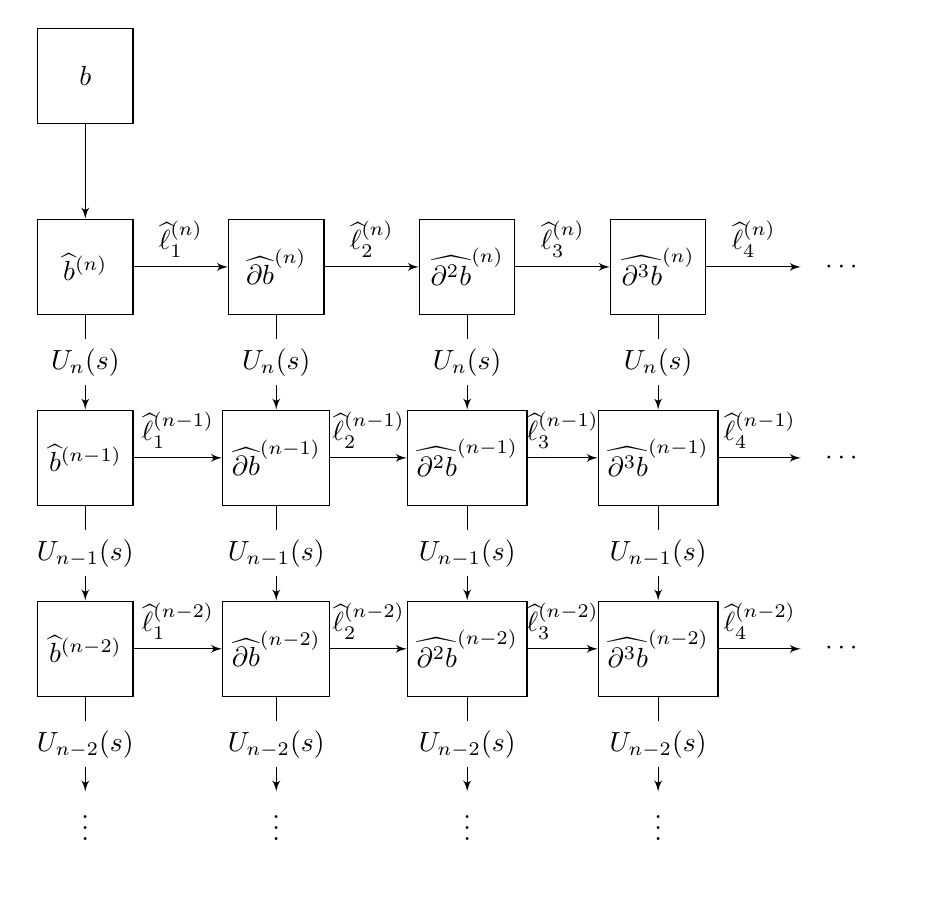
\begin{tikzpicture}[node distance = 0.2\textwidth]
    \node [box] (bj) {\(b\)};
    \node [box, below of=bj] (bn0) {\(\widehat{b}^{(n)}\)};
    \node [box, right of=bn0] (dbn0) {\(\widehat{\partial b}^{(n)}\)};
    \node [box, right of=dbn0] (ddbn0) {\(\widehat{\partial^2 b}^{(n)}\)};
    \node [box, right of=ddbn0] (dddbn0) {\(\widehat{\partial^3 b}^{(n)}\)};
    %%
    \node [box, below of=bn0] (bn1) {\(\widehat{b}^{(n - 1)}\)};
    \node [box, below of=dbn0] (dbn1) {\(\widehat{\partial b}^{(n - 1)}\)};
    \node [box, below of=ddbn0] (ddbn1) {\(\widehat{\partial^2 b}^{(n - 1)}\)};
    \node [box, below of=dddbn0] (dddbn1) {\(\widehat{\partial^3 b}^{(n - 1)}\)};
    %%
    \node [box, below of=bn1] (bn2) {\(\widehat{b}^{(n - 2)}\)};
    \node [box, below of=dbn1] (dbn2) {\(\widehat{\partial b}^{(n - 2)}\)};
    \node [box, below of=ddbn1] (ddbn2) {\(\widehat{\partial^2 b}^{(n - 2)}\)};
    \node [box, below of=dddbn1] (dddbn2) {\(\widehat{\partial^3 b}^{(n - 2)}\)};
    %%
    \path [line] (bn0) -- node[above] {\(\widehat{\ell}_1^{(n)}\)} (dbn0);
    \path [line] (dbn0) -- node[above] {\(\widehat{\ell}_2^{(n)}\)} (ddbn0);
    \path [line] (ddbn0) -- node[above] {\(\widehat{\ell}_3^{(n)}\)} (dddbn0);
    \node [empty-box, right of=dddbn0] (right0) {\(\cdots\)};
    \path [line] (dddbn0) -- node[above] {\(\widehat{\ell}_4^{(n)}\)} (right0);
    %%
    \path [line] (bn1) -- node[above] {\(\widehat{\ell}_1^{(n - 1)}\)} (dbn1);
    \path [line] (dbn1) -- node[above] {\(\widehat{\ell}_2^{(n - 1)}\)} (ddbn1);
    \path [line] (ddbn1) -- node[above] {\(\widehat{\ell}_3^{(n - 1)}\)} (dddbn1);
    \node [empty-box, right of=dddbn1] (right1) {\(\cdots\)};
    \path [line] (dddbn1) -- node[above] {\(\widehat{\ell}_4^{(n - 1)}\)} (right1);
    %%
    \path [line] (bn2) -- node[above] {\(\widehat{\ell}_1^{(n - 2)}\)} (dbn2);
    \path [line] (dbn2) -- node[above] {\(\widehat{\ell}_2^{(n - 2)}\)} (ddbn2);
    \path [line] (ddbn2) -- node[above] {\(\widehat{\ell}_3^{(n - 2)}\)} (dddbn2);
    \node [empty-box, right of=dddbn2] (right2) {\(\cdots\)};
    \path [line] (dddbn2) -- node[above] {\(\widehat{\ell}_4^{(n - 2)}\)} (right2);
    %%
    \path [line] (bj) -- (bn0);
    \path [line] (bn0) -- node[fill=white] {\(U_n(s)\)} (bn1);
    \path [line] (bn1) -- node[fill=white] {\(U_{n - 1}(s)\)} (bn2);
    \node [empty-box-vert, below of=bn2] (bottom0) {\(\vdots\)};
    \path [line] (bn2) -- node[fill=white] {\(U_{n - 2}(s)\)} (bottom0);
    %%
    \path [line] (dbn0) -- node[fill=white] {\(U_n(s)\)} (dbn1);
    \path [line] (dbn1) -- node[fill=white] {\(U_{n - 1}(s)\)} (dbn2);
    \node [empty-box-vert, below of=dbn2] (bottom1) {\(\vdots\)};
    \path [line] (dbn2) -- node[fill=white] {\(U_{n - 2}(s)\)} (bottom1);
    %%
    \path [line] (ddbn0) -- node[fill=white] {\(U_n(s)\)} (ddbn1);
    \path [line] (ddbn1) -- node[fill=white] {\(U_{n - 1}(s)\)} (ddbn2);
    \node [empty-box-vert, below of=ddbn2] (bottom2) {\(\vdots\)};
    \path [line] (ddbn2) -- node[fill=white] {\(U_{n - 2}(s)\)} (bottom2);
    %%
    \path [line] (dddbn0) -- node[fill=white] {\(U_n(s)\)} (dddbn1);
    \path [line] (dddbn1) -- node[fill=white] {\(U_{n - 1}(s)\)} (dddbn2);
    \node [empty-box-vert, below of=dddbn2] (bottom3) {\(\vdots\)};
    \path [line] (dddbn2) -- node[fill=white] {\(U_{n - 2}(s)\)} (bottom3);
\end{tikzpicture}
\caption{Filtering errors}
\end{figure}

\section{Numerical experiments}\label{sec:numerical}

\begin{figure}[H]
  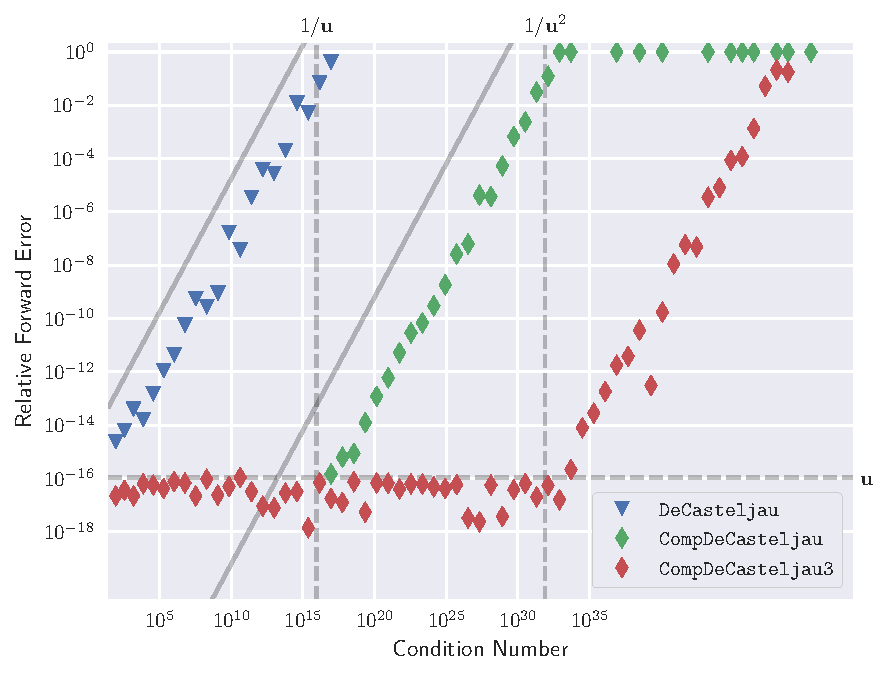
\includegraphics[width=0.8125\textwidth]{../images/de_casteljau_rel_error.pdf}
  \centering
  \caption{Accuracy of evaluation of \(p(s) = (s - 1)\left(s - 3/4\right)^7\)
    represented in Bernstein form.}
\end{figure}

\section{IEEE Stuff}

\begin{algorithm}[H]
  \caption{\textit{EFT of the sum of two floating point numbers.}}

  \begin{algorithmic}
    \Function{\(\left[S, \sigma\right] = \mathtt{TwoSum}\)}{$a, b$}
      \State \(S = a \oplus b\)
      \State \(z = S \ominus a\)
      \State \(\sigma = (a \ominus (S \ominus z)) \oplus (b \ominus z)\)
    \EndFunction
  \end{algorithmic}
\end{algorithm}

\begin{algorithm}[H]
  \caption{\textit{Splitting of a floating point number into two parts.}}

  \begin{algorithmic}
    \Function{\(\left[h, \ell\right] = \mathtt{Split}\)}{$a$}
      \State \(z = a \otimes (2^r + 1)\)
      \State \(h = z \ominus (z \ominus a)\)
      \State \(\ell = a \ominus h\)
    \EndFunction
  \end{algorithmic}
\end{algorithm}

\begin{algorithm}[H]
  \caption{\textit{EFT of the product of two floating point numbers.}}

  \begin{algorithmic}
    \Function{\(\left[P, \pi\right] = \mathtt{TwoProd}\)}{$a, b$}
      \State \(P = a \otimes b\)
      \State \(\left[a_h, a_{\ell}\right] = \mathtt{Split}(a)\)
      \State \(\left[b_h, b_{\ell}\right] = \mathtt{Split}(b)\)
      \State \(\pi = a_{\ell} \otimes b_{\ell} \ominus (((P \ominus
          a_h \otimes b_h)
          \ominus a_{\ell} \otimes b_h) \ominus a_h \otimes b_{\ell})\)
    \EndFunction
  \end{algorithmic}
\end{algorithm}

\begin{algorithm}[H]
  \caption{\textit{EFT of the sum of two floating point numbers with a FMA.}}

  \begin{algorithmic}
    \Function{\(\left[P, \pi\right] = \mathtt{TwoProdFMA}\)}{$a, b$}
      \State \(P = a \otimes b\)
      \State \(\pi = \mathtt{FMA}(a, b, -P)\)
    \EndFunction
  \end{algorithmic}
\end{algorithm}

\section{de Casteljau's Method}

Consider de Casteljau's method to evaluate a degree \(n\)
polynomial in Bernstein-B\'{e}zier form with control points \(b_j\):
\begin{align}
    b_j^{(n)} &= b_j \\
    b_j^{(k)} &= (1 - s) b_j^{(k + 1)} + s b_{j + 1}^{(k + 1)} \\
    b(s) &= b_0^{(0)}.
\end{align}

\subsection{Condition Number}

For a polynomial \(p(x)\) in the power basis, we have
(\cite{langlois_et_al:DSP:2006:442}):
\begin{equation}
\cond{p(x)} = \frac{\widetilde{p}\left(\left|x\right|\right)}{
  \left|p(x)\right|} = \frac{\sum_j \left|a_j\right| \left|x\right|^j}{
  \left|p(x)\right|}.
\end{equation}
In particular, this means that if \(x \geq 0\) and each \(a_j \geq 0\)
we must necessarily have \(\cond{p(x)} = 1\). To see an example in use,
consider \(p(x) = (x - 1)^n\) and input values of the form \(x = 1 + \delta\)
(with \(\left|\delta\right| \ll 1\)). Since \(a_j = \binom{n}{j} (-1)^{n - j}\)
we have \(\widetilde{p}(x) = (x + 1)^n\) hence
\begin{equation}
\cond{p\left(1 + \delta\right)} = \frac{(2 + \delta)^n}{
  \left|\delta\right|^n} = \left|1 + \frac{2}{\delta}\right|^n.
\end{equation}
As \(\delta \to 0\), this value approaches \(\infty\) (as expected).

For a polynomial \(p(s)\) in Bernstein form, we have (\cite{Jiang2010}):
\begin{equation}
\cond{p(s)} = \frac{\widetilde{p}\left(s\right)}{
  \left|p(s)\right|} = \frac{\sum_j \left|b_j\right| \left|B_{j, n}(s)\right|}{
  \left|p(s)\right|}.
\end{equation}
The Bernstein form is suited for \(s \in \left[0, 1\right]\), which means
\(B_{j, n}(s) \geq 0\) typically. If \(s \in \left[0, 1\right]\) and each
\(b_j \geq 0\) we must necessarily have \(\cond{p(s)} = 1\). To see an
example in use, consider
\begin{equation}
p(s) = (1 - 2s)^n = \left[(1 - s) - s\right]^n = \sum_j \binom{n}{j}
(1 - s)^{n - j} (-s)^j = \sum_j (-1)^j B_{j, n}(s)
\end{equation}
and input values of the form \(x = \frac{1}{2} + \delta\)
(with \(\left|\delta\right| \ll \frac{1}{2}\)). Since \(b_j = (-1)^j\)
we have \(\widetilde{p}(s) = \left[(1 - s) + s\right]^n = 1\)
\begin{equation}
\cond{p\left(\frac{1}{2} + \delta\right)} = \frac{1}{
  \left|2\delta\right|^n}.
\end{equation}
As \(\delta \to 0\), this value approaches \(\infty\) (as expected).

\subsection{Example of Compensated de Casteljau Failing}

Consider
\begin{equation}
p(s) = (4s - 3)^3 (8s + 7) = (-189) B_{0, 4}(s) + (-54) B_{1, 4}(s) +
57 B_{2, 4}(s) + (-32) B_{3, 4}(s) + 15 B_{4, 4}(s)
\end{equation}
at the point \(s = \frac{3}{4} + 800 \mach\). In exact arithmetic, we
have \(p(s) = 13(3200\mach)^3 + \mathcal{O}\left(\mach^4\right)\).
However, using the compensated de Casteljau algorithm results in
\(\widehat{b}_0^{(0)} \oplus \widehat{\partial b}_0^{(0)} = 0\):

\begin{center}
  \begin{tabular}{>{$}c<{$} >{$}c<{$} >{$}c<{$} >{$}c<{$} >{$}c<{$} >{$}c<{$}}
    \toprule
    k & j & \widehat{b}_j^{(k)} & \widehat{\partial b}_j^{(k)} & \widehat{\partial^2 b}_j^{(k)} & \widehat{\partial^3 b}_j^{(k)} \\
    \midrule
    3 & 0 & -87\frac{3}{4} + 108032\mach & -32\mach & 0 & 0 \\
    3 & 1 & 29\frac{1}{4} + 88768\mach & 32\mach & 0 & 0 \\
    3 & 2 & -9\frac{3}{4} - 71200\mach & 0 & 0 & 0 \\
    3 & 3 & 3\frac{1}{4} + 37600\mach & 0 & 0 & 0 \\
    \midrule
    2 & 0 & 187200\mach & -15360000\mach^2 & 0 & 0 \\
    2 & 1 & -62408\mach & 8\mach - 128000000\mach^2 & 0 & 0 \\
    2 & 2 & 20800\mach & 87040000\mach^2 & 0 & 0 \\
    \midrule
    1 & 0 & -6\mach - 199688192\mach^2 & 6\mach - 99831808\mach^2 & -90112000000\mach^3 & 0 \\
    1 & 1 & -2\mach + 66568192\mach^2  & 2\mach + 33271808\mach^2 & 172032000000\mach^3 & 0 \\
    \midrule
    0 & 0 & -3\mach + 7296\mach^2 & 3\mach - 7296\mach^2 & 13 (3200\mach)^3 + 3048(512\mach)^4 & 962(128\mach)^4 \\
    \bottomrule
  \end{tabular}
\end{center}

\subsection{Selection of Test Cases}

From \cite{Delgado2015} (end of Section 3):

\begin{quote}
  We can observe that, in this case, the algorithm with a good
  behavior everywhere is the de Casteljau algorithm
\end{quote}

\noindent In the same paper (when referring to \cite{Bezerra2013} at the
beginning of Section 2):

\begin{quote}
  assuming that all control points are positive. This assumption avoided
  ill-conditioned polynomials. In this section, we shall show that this is
  a natural assumption in Computer Aided Geometric Design (from now on,
  C.A.G.D.) and that it permits to assure high relative precision for the
  evaluation through a large family of representations in C.A.G.D.
\end{quote}

\noindent From the same author, in \cite{Mainar2005} (towards the
end of Section 5, at the bottom of page 109):

\begin{quote}
  Let us observe that in this case, the de Casteljau algorithm presents
  better stability properties for the evaluation near the roots. In fact,
  the de Casteljau algorithm has good behaviour even when using simple
  precision, although the running error bound is not so accurate in points
  close to the roots.
\end{quote}

\subsection{Operation Counts}

After implementing for \(K = 2, 3, \ldots, 12\) and instrumenting all
relevant floating point operations, the \(K\)-fold Horner requires
\begin{equation}
(5 \cdot 2^K - 8)n + \left((K + 8) 2^K - 12K - 6\right) =
\mathcal{O}\left((n + K)2^K\right)
\end{equation}
flops to evaluate a degree \(n\) polynomial (this only applies when
\(n \geq K - 1\)). As a comparison, the
non-compensated form of Horner requires \(2n\) flops. Of these,
\(\left(2^{K - 1} - 1\right)n - 2^{K - 1}(K - 3) - 2\) are
FMA (fused-multiply-add) instructions.

After implementing for \(K = 2, 3, 4, 5\) and instrumenting all relevant
floating point operations, the \(K\)-fold de Casteljau requires
\begin{equation}
(15K^2 - 34K + 26)T_n + K + 5 =
\mathcal{O}\left(n^2 K^2\right)
\end{equation}
flops to evaluate a degree \(n\) polynomial. (Here \(T_n\) is the
\(n\)th triangular number.) As a comparison, the non-compensated form of
de Casteljau requires \(3 T_n + 1\) flops. Of these, \((3K - 4)T_n\) are
FMA instructions. On hardware that doesn't support FMA,
every FMA will be exchanged for 10 \(\ominus\)'s and 6 \(\otimes\)'s so the
count will increase by \((10 + 6 - 1)(3K - 4)T_n\).

\section{Bogus Section for Refs}

Here they are, for now
\begin{itemize}
  \item Newton with compensated Horner (\cite{Graillat2008})
\end{itemize}

\bibliography{paper}
\bibliographystyle{alpha}

\end{document}
